\documentclass[10pt,oneside,letterpaper,article]{memoir}

% the memoir class is an extremely flexable and scalable
% package for document layout. The memoir manual:

%    http://tug.ctan.org/tex-archive/macros/latex/contrib/memoir/memman.pdf

% is very well written and extremely detailed.

%%%%%%%%%%%%%%%%%%%%%%%%%%%%%%%
%
%
% Begin Document Header Here
%
%
%%%%%%%%%%%%%%%%%%%%%%%%%%%%%%%

%%------------Packages

%%------------column layout
\usepackage{multicol}
% Figures within a column...
\makeatletter
\newenvironment{tablehere}
{\vskip\onelineskip%
\def\@captype{table}}
{}
\newenvironment{figurehere}
{\vskip\onelineskip%
\def\@captype{figure}}
{}
\makeatother

%%------------mathmatical support
\usepackage{amsmath}
\usepackage{amssymb}

%%------------graphics
\usepackage{graphicx}

%%------------nomenclature
\usepackage{nomencl}
\makenomenclature
\usepackage{ifthen}
% Indent nomenclature entries
\renewcommand{\nomlabel}[1]{\hfill #1\ }

%%------------bibliography
\usepackage{natbib}
\bibliographystyle{agufull04}


%%------------a selection of font packages
% see http://www.tug.dk/FontCatalogue/ for a complete description of commonly
% available LaTeX fonts.

%\usepackage[scaled=.9]{couriers}
%\usepackage{pxfonts}
\usepackage{mathpazo}
%\usepackage{mathpple}
%\usepackage{fouriernc}
%\usepackage[garamond]{mathdesign}
%\usepackage{kurier}

%%-----------realias traditional LaTeX font style commands
\renewcommand{\it}{\itshape}
\renewcommand{\sl}{\slshape}
\renewcommand{\bf}{\bfseries}
\renewcommand{\sf}{\sffamily}
\renewcommand{\tt}{\ttfamily}

%%-----------set title information
\title{Another Research Paper}
\author{A. Student}
\newcommand{\theInstitution}{Department of Environmental Resources Engineering, Humboldt State University, Arcata, California 95521}
\newcommand{\theClass}{Engr Whatever: Another Engineering Class}
\date{\today}

%%------------page setup

% Define text width by setting right and left margins
\setlrmarginsandblock{0.75in}{0.75in}{*}
% Define text height by setting upper and lower margins
\setulmarginsandblock{0.75in}{1.25in}{*}
% These define the distance from the type block of the header and footer
\setheadfoot{\baselineskip}{0.25in}
\setheaderspaces{*}{0.25in}{*}
\checkandfixthelayout
%%----------See page p. 72 of the memoir manual for more page formatting options


%%-----------If weird gaps appear on a page enable this
%\raggedbottom

%%-----------causes chapter headings to behave like section headings
% I.E, no page break before new chapters.
\chapterstyle{article}

%%----------fine tuning of chapter styles
\setlength{\beforechapskip}{\baselineskip}
\setlength{\afterchapskip}{0.5em}
\renewcommand{\chaptitlefont}{\large\bfseries}

%%----------fine tuning of section styles
\setbeforesecskip{0.5em}
\setaftersecskip{0.25em}
\setsecheadstyle{\normalsize\bfseries}

%%----------fine tuning of subsection styles
\setbeforesubsecskip{0.05em}
\setaftersubsecskip{0.05em}
\setsubsecheadstyle{\normalsize\bfseries}

%%----------See page p. 152 of the memoir manual for more section formatting options

%%-----------include every header subsubsection level and above
% in the numbering scheme and the table of contents.
\setsecnumdepth{subsection}
\settocdepth{subsection}


%%-----------set header and footer styles
\makepagestyle{firstPage}
	\makeoddhead{firstPage}{}{\scshape\theClass\quad\thedate}{}
	\makeoddfoot{firstPage}{}{\thepage}{}
\makepagestyle{otherPages}
	\makeevenhead{otherPages}{\scshape\thepage}{\scshape\theauthor :\quad\thetitle}{}
	\makeoddhead{otherPages}{}{\scshape\theauthor :\quad\thetitle}{\scshape\thepage}

%%----------See page p. 166 of the memoir manual for more header/footer formatting options


%%-----------set the style of figure and table captions
\captionnamefont{\bfseries}


%%----------useful macros

% Derivatives and partial derivatives
\newcommand{\deriv}[3][]{\ensuremath{\frac{d^{#1} #2}{d #3^{#1}}}}
\newcommand{\pderiv}[3][]{\ensuremath{\frac{\partial ^{#1} #2}{\partial #3^{#1}}}}

%% nice inline fractions
\newcommand{\slanty}[2]{$^{#1}\!\!\hspace{1pt}/\hspace{2pt}\!\!_{#2}$\!\!\!\hspace{4pt}}

% New list of variables environment which is automagically copied to the
% table of nomenclature

\newenvironment{variables}%
  {\noindent where:\begin{itemize}}%
  {\end{itemize}}%
  
\newcommand{\var}[3][]{\ifthenelse{\equal{#1}{}}%
  {\item[\ensuremath{#2}]{#3}\nomenclature{\ensuremath{#2}}{#3}}%
  {\item[\ensuremath{#2}]{#3}\nomenclature{\ensuremath{#2}}{#1}}}

%%%%%%%%%%%%%%%%%%%%%%%%%%%%%%%
%
%
% End Document Header Here
%
%
%%%%%%%%%%%%%%%%%%%%%%%%%%%%%%%

%%%%%%%%%%%%%%%%%%%%%%%%%%%%%%%
%
%
% Document Starts Here
%
%
%%%%%%%%%%%%%%%%%%%%%%%%%%%%%%%
\begin{document}

% The header style used for the entire document is otherPages
\pagestyle{otherPages}
% However, for the very first page, the firstPage style is used
\thispagestyle{firstPage}

% Drop the title by 0.25 in
\vskip 0.25in

% Print out title information
{\noindent\LARGE\bfseries\thetitle}\vskip\onelineskip
\noindent\theauthor\\
{\footnotesize\noindent\theInstitution}\\


%%-----------set the abstract format

% Place the abstract tile inline with the text
	\abstractrunin
%Don't indent the abstract tiltle
	\setlength{\abstitleskip}{-\absparindent}
%Follow the abstract title with a period and a quad space
	\abslabeldelim{.\quad}
%Align the left edge of the abstract with the body text
	\setlength{\absleftindent}{0in}
%Set the right edge of the abstract back one inch from the body text
	\setlength{\absrightindent}{1in}
%%----------See page p. 117 of the memoir manual for more abstract formatting options

\begin{abstract}
Lorem ipsum dolor sit amet, consectetur adipiscing elit. Ut fringilla fermentum velit. Nulla facilisi. Vivamus sit amet eros. Ut molestie nulla nec quam. Nam pellentesque. Nam consequat elementum quam. Donec nibh ligula, dignissim non, fringilla vitae, tempus placerat, purus. Suspendisse tempor erat in turpis condimentum semper. Fusce dictum. Donec at arcu quis orci congue dapibus. Quisque et ante. Donec lobortis, dui dictum lacinia commodo, turpis nisl aliquet tortor, nec scelerisque risus enim quis ante. Nam lobortis dui. Sed pretium orci.

Pellentesque laoreet, sapien ut elementum porttitor, enim neque eleifend arcu, non auctor sapien dui nec sem. In sollicitudin dolor et nulla. Nunc cursus metus sed urna. Suspendisse potenti. Ut tortor arcu, vestibulum ut, porta ut, tincidunt sed, tellus. Maecenas leo. Duis auctor augue. Vestibulum erat odio, mollis id, dapibus id, cursus eu, lorem. Vestibulum vehicula. Ut et leo nec erat pellentesque tincidunt. Donec lacinia lacus et nisi. Fusce lobortis, felis laoreet aliquet venenatis, eros leo vulputate nulla, id vulputate arcu felis sit amet quam. Nam a tellus eget orci lacinia gravida.

\end{abstract}\vskip\onelineskip

%%-----------begin document body- set in two columns
\begin{multicols*}{2}
\chapter{Introduction}

Phasellus hendrerit erat sit amet enim. Maecenas volutpat mattis mauris. Fusce dignissim mauris nec felis. Ut accumsan ipsum eget velit. Cras enim. Aliquam erat volutpat. Sed sem justo, lacinia non, scelerisque ac, viverra sit amet, metus. Quisque vitae tortor quis arcu pharetra bibendum. Suspendisse scelerisque, nibh eu placerat consectetur, nisl diam accumsan risus, ut aliquam tellus massa sit amet sapien. Aliquam non odio. Vestibulum elit massa, scelerisque sit amet, mollis vel, imperdiet tincidunt, magna. Nam ac turpis. Morbi eros tortor, lobortis id, dignissim in, tincidunt in, libero. Suspendisse sed metus. Cras ipsum. Vestibulum ante ipsum primis in faucibus orci luctus et ultrices posuere cubilia Curae.

\section{Vivamus at est}
\subsection{Curabitur tempus velit at mauris}
Cras eget nulla quis velit aliquet sagittis. Fusce in arcu non lectus dictum pulvinar. Sed purus massa, consectetur nec, ullamcorper ut, imperdiet quis, ligula. Cras sed nunc. Suspendisse vulputate metus vel urna. Quisque congue adipiscing elit. 

\begin{itemize}
 
 \item{Nulla facilisis est sed felis.}
  
 \item{Donec fermentum varius tortor.}
  
 \item{Morbi blandit laoreet felis.}
 
\end{itemize}

Nam tempus tempus justo. Ut ligula nisi, mollis ut, congue eu, lobortis in, est. Praesent faucibus condimentum orci. Pellentesque eu lorem in diam sollicitudin congue. In elementum varius arcu. Suspendisse potenti. Phasellus at libero sed turpis venenatis varius. Quisque magna. Duis sed diam. Aenean aliquam enim nec est.

\subsection{Aenean a nulla}
Pellentesque semper, elit et fringilla feugiat, purus ligula fermentum sem, et dictum elit massa a sapien. Aliquam ultrices leo vel neque tristique hendrerit. Nam sed orci. Donec est. Nullam sed ipsum eu lacus gravida laoreet. Sed non ligula at velit pulvinar elementum. Nulla tortor augue, sodales vel, auctor id, vulputate eget, purus. Quisque in mi. Aenean iaculis leo eu nibh. Donec porta sem nec dui. Etiam pretium interdum nunc. Mauris nulla. Duis accumsan, dolor at pellentesque ultrices, diam erat consequat massa, dictum volutpat diam ante eget mauris. Quisque euismod ante a lorem. Aliquam nec est.

\begin{figure*}[!b]
  \centering
  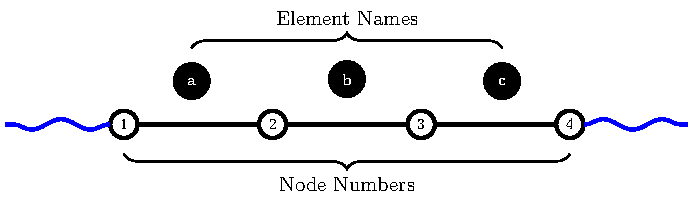
\includegraphics{figs/finEle.pdf}
 \caption{Two-column figure.}
\end{figure*}

\chapter{Problem Formulation}

Vestibulum pellentesque arcu. Aliquam quam ligula, consectetur quis, ornare vel, lacinia eget, velit. Donec eget lacus. Cras nec nisi quis dolor bibendum tristique. Duis tincidunt ornare dui. Suspendisse lobortis. Phasellus egestas lacus vitae arcu egestas pharetra. Cras rhoncus augue eu nisl. Morbi sed nisi. Pellentesque ac tellus. Fusce eu sem nec diam gravida posuere. Nulla facilisi. Aliquam rhoncus arcu ut enim. Quisque gravida interdum tellus. Phasellus ornare. Aenean luctus feugiat urna. Aliquam ultrices urna sit amet nunc. Morbi vestibulum ante. Nunc posuere \citep{bear72}.

\begin{equation} 
  \vec{q}=-k\nabla\cdot h
\end{equation}

% The variables environment will list variable names in an itemized list beginning with
% where. The variables will also be echoed into the nomenclature list at the end of the
% document.
\begin{variables}
  \var{\vec{q}}{A vector of flow rates. }
  
  \var{k}{Hydraulic conductivity.}
  
  \var{h}{Hydraulic head in meters.}
  
  % This variable has an alternate description that will appear in the
  % nomenclature section
  \var[Funky symbol isn't it?]{\nabla}{A vector of partial derivatives.}
  
\end{variables}

Integer iaculis consequat dolor. Nunc sapien mi, egestas sit amet, dictum nec, pellentesque ut, massa. Cum sociis natoque penatibus et magnis dis parturient montes, nascetur ridiculus mus. Maecenas tortor nunc, gravida ut, posuere vitae, elementum eget, nisi. Nunc dapibus vulputate diam. In sodales. Cras tincidunt suscipit tortor. Suspendisse vehicula nibh quis libero. Vestibulum neque augue, condimentum eu, ornare id, tempus et, metus. Sed vehicula lacus in elit. Donec mauris. Nullam ac felis. Nam mauris diam, aliquam vel, feugiat in, cursus sed, turpis. Pellentesque dignissim viverra nisl. Nullam sem sem, faucibus non, eleifend sed, ornare ac, lacus. Fusce vulputate nunc non nulla. Quisque ligula leo, eleifend sed, cursus ut, congue lacinia, sapien.


% Example of a long equation which needs to be broken over several lines
% the multline environment is part of amsmath.
\begin{multline}
 \pderiv{}{x}\left( K_{x}h\pderiv{h}{x}\right) +
 \pderiv{}{y}\left( K_{y}h\pderiv{h}{y}\right) +\\ % Note the line break!
 \pderiv{}{y}\left( K_{z}h\pderiv{h}{z}\right) \pm Q
 = S_{y}\pderiv{h}{t}
\end{multline}


Duis gravida, sapien eu porttitor adipiscing, tortor quam sollicitudin ipsum, sit amet condimentum nisl urna ut ante. Nullam eros neque, volutpat at, convallis eget, congue viverra, elit. Nulla imperdiet. Duis eros nisi, rutrum et, interdum sit amet, placerat vitae, felis. Sed aliquet mauris nec turpis. Phasellus nibh quam, venenatis at, consectetur et, mollis a, diam. Vivamus vel sapien non libero ornare vestibulum. Donec placerat arcu sit amet ipsum. Pellentesque non turpis accumsan nisi molestie aliquet. Maecenas varius dolor ac est. Sed pretium, ante et dictum pretium, erat libero varius diam, tristique molestie risus justo et felis. Donec neque. Cras elementum porttitor eros. Donec sodales turpis at dui facilisis gravida. Donec non justo. Nunc viverra aliquet libero.

\chapter{Literature Review}

Praesent non mi. Mauris rhoncus. Praesent odio metus, feugiat eu, vehicula id, pretium ac, sapien. Aenean eget ante. Integer faucibus tellus non erat. Proin nibh nisl, aliquam eget, pretium id, fermentum at, ante. Etiam quam turpis, dapibus id, viverra quis, ullamcorper in, elit. Nullam in nisi eget nisl aliquam vestibulum. Sed non ligula vel massa dapibus pulvinar. Nulla ut mauris in mi sodales commodo. In venenatis pharetra ligula. Phasellus luctus elit placerat sapien. Donec eros. Aliquam feugiat. Vestibulum in odio. Proin hendrerit, orci ut faucibus mattis, quam arcu blandit justo, quis mollis velit nunc quis libero.

Cras tempor porta risus. Nulla pellentesque magna sit amet ante. Sed vehicula risus in velit. Fusce in diam sit amet neque imperdiet mollis. Mauris eget nisi condimentum justo fringilla mattis. In hac habitasse platea dictumst. Lorem ipsum dolor sit amet, consectetur adipiscing elit. In nibh. Morbi vitae nunc. Phasellus orci purus, fermentum at, ultricies vehicula, laoreet et, enim. Vestibulum ante ipsum primis in faucibus orci luctus et ultrices posuere cubilia Curae; Lorem ipsum dolor sit amet, consectetur adipiscing elit. Fusce id ipsum id urna fringilla elementum. Vivamus dignissim. Quisque sollicitudin. In hac habitasse platea dictumst.

\begin{figurehere}
 \centering
 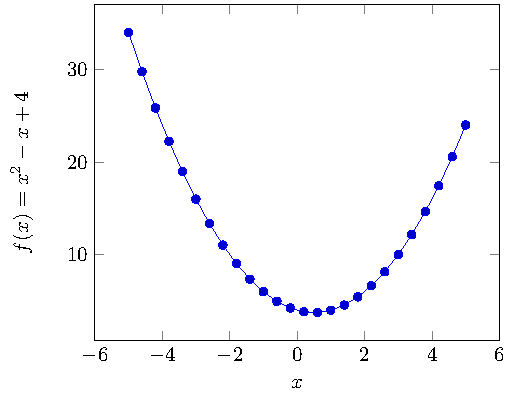
\includegraphics{figs/plot.pdf}
 \caption{One-column figure.}
\end{figurehere}

Nullam magna ante, semper ut, egestas id, auctor convallis, dui. Vivamus nibh. Curabitur dignissim libero sed magna. Suspendisse orci arcu, condimentum ac, posuere laoreet, consequat a, metus. Integer vehicula velit sit amet odio. Sed sollicitudin, felis et faucibus viverra, nisl elit gravida massa, et mollis enim nibh non est. Nulla in lacus. Nunc accumsan, mauris vitae pellentesque rhoncus, velit mauris pretium mi, sed interdum arcu lacus eu tortor. Morbi ac quam. Vivamus vitae quam eleifend massa aliquam luctus. Duis tincidunt dignissim turpis. Maecenas feugiat tempus urna. Vivamus mollis commodo lectus. 

\printnomenclature

\bibliography{bibliography}

\end{multicols*}


%%%%%%%%%%%%%%%%%%%%%%%%%%%%%%%
%
%
% Document Ends Here
%
%
%%%%%%%%%%%%%%%%%%%%%%%%%%%%%%%

\end{document}